\documentclass[journal=tches,final]{iacrtrans}
\usepackage{algorithm}
\usepackage{algpseudocode}
\usepackage{graphicx}
\usepackage{booktabs}
\usepackage{multirow}
\usepackage{lipsum}
\usepackage{tikz}
\usetikzlibrary{patterns}
\usetikzlibrary{arrows}
\usepackage{float}
\usepackage{subcaption}
\usepackage{xcolor}
\usepackage{caption}
\usepackage{pgf}

\newcommand{\mathdefault}[1][]{#1}
\raggedbottom

\begin{document}

\title{Side-channel Attacks on SIMON Block Cipher: \\ CPA and Leakage Assessment on unprotected and masked implementations}

\author{
    Nico Makowe \and
    Kandarp Lalit\and
    Majdi Maraqa}

\date{\today}
\institute{
	Hochschule Albstadt-Sigmaringen, Albstadt-Ebingen, Germany
	\email[makoweni@hs-albsig.de,lalitkan@hs-albsig.de,maraqama@hs-albsig.de]{{makoweni,lalitkan,maraqama}@hs-ablsig.de}
}

\maketitle
\fancyhead[RE]{Side-channel Attacks on SIMON Block Cipher}


\begin{abstract}
This paper investigates implementation-level vulnerabilities of the lightweight block cipher SIMON by means of power-based side-channel analysis. A software implementation on an embedded ARM Cortex-M4 target is analyzed, demonstrating that measuring power consumption enables key recovery using Correlation Power Analysis (CPA). To mitigate these vulnerabilities, boolean masking is implemented. Welch's t-test was performed for statistical leakage assessment. The results show high leakage in the unprotected implementation and significantly lower t-values in the masked implementation. These findings emphasize the importance of careful countermeasure design in lightweight cryptographic implementations.

\keywords{lightweight cryptography, side-channel analysis, correlation power analysis, SIMON, masking, implementation security, ChipWhisperer}
\end{abstract}

\section{Introduction}
Lightweight cryptography plays a crucial role in securing resource-constrained devices in the Automotive and IoT industry, where limitations in memory, power consumption, and computational capabilities must be carefully considered. The SIMON block cipher, introduced by the National Security Agency in 2013, is a family of lightweight block ciphers designed to achieve high performance in hardware while remaining efficient in software implementations.

SIMON, like many cryptographic algorithms, is susceptible to implementation-level attacks. In particular, side-channel attacks exploit physical leakage such as power consumption or electromagnetic radiation to recover secret information without breaking the underlying cryptographic primitive.

This paper investigates Correlation Power Analysis (CPA) applied to a software implementation of SIMON. Furthermore, the masking countermeasure is analyzed and its effectiveness in increasing resistance against power-based attacks is evaluated. The presented work follows a systematic attack-and-evaluation methodology commonly used in the analysis of cryptographic implementations.

\paragraph{The Simon Block Cipher}
Simon is a family of lightweight block ciphers based on a Feistel structure. The cipher supports multiple configurations with block sizes of 32, 48, 64, 96, and 128 bits, and key sizes ranging from 64 to 256 bits. \cite{beaulieu2015simon}

This study focuses on Simon-64/128, which operates on 64-bit blocks using a 128-bit key over 44 rounds. The cipher is designed for optimal performance in both hardware and software implementations, featuring only bitwise XOR, AND, and rotation operations.

The round function for Simon-64/128 is defined as:
\[
R_k(x, y) = (y \oplus f(x) \oplus k, x)
\]
where 
\[
f(x) = (S^1(x) \& S^8(x)) \oplus S^2(x)
\]
Here, \(S^j\) denotes left circular shift by \(j\) bits, \(\oplus\) represents bitwise XOR, \(\&\) denotes bitwise AND, and \(k\) is the round key derived from the master key through a key schedule.

\begin{figure}[ht]
    \centering
    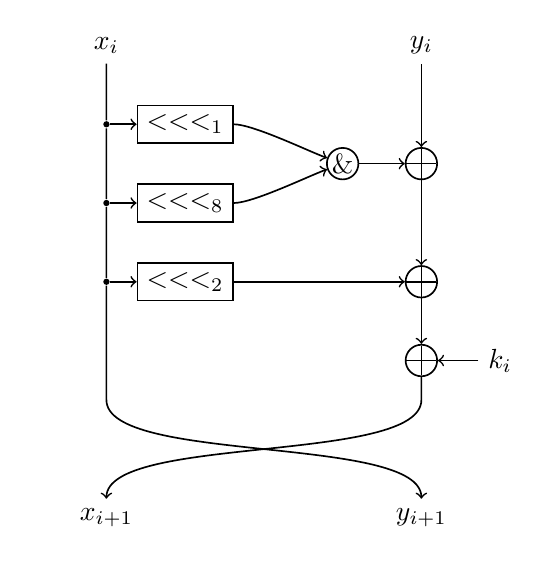
\begin{tikzpicture}
	[line width=0.6,trim left,
	box/.style = {
		draw
	},
	loosewire/.style = {
		looseness=0.5,
	},
	xor/.style = {
		draw, circle, inner sep=0cm, minimum size=0.4cm,
		append after command = {
			[shorten >=\pgflinewidth, shorten <=\pgflinewidth,]
			(\tikzlastnode.north) edge (\tikzlastnode.south)
			(\tikzlastnode.east) edge (\tikzlastnode.west)
		}
	},
	odot/.style = {
		draw, circle, inner sep=0cm, minimum size=0.4cm
	},
	dot/.style = {
		fill, circle, inner sep=0cm, minimum size=0.08cm
	},
	invisible/.style = {
		minimum size=0cm
	}]
	
	%Draw nodes
	\node at (1,7) (xin) {$x_i$};
	\node at (5,7) (yin) {$y_i$};
	\node[dot] at (1,6) (d1) {};
	\node[dot] at (1,5) (d2) {};
	\node[dot] at (1,4) (d3) {};
	\node[box] at (2,6) (S1) {$<<<_1$};
	\node[box] at (2,5) (S2) {$<<<_8$};
	\node[box] at (2,4) (S3) {$<<<_2$};
	\node[xor] at (5,5.5) (x1) {};
	\node[xor] at (5,4) (x2) {};
	\node[xor] at (5,3) (x3) {};
	\node[odot] at (4,5.5) (AND) {$\&$};
	\node at (6,3) (k) {$k_i$};
	\node at (1, 1) (xout) {$x_{i+1}$};
	\node at (5, 1) (yout) {$y_{i+1}$};
	\coordinate (cright) at (5, 2.5);
	\coordinate (cleft) at (1, 2.5);
	
	%Draw wires
	\draw[->] (d1) -- (S1);
	\draw[loosewire,->] (S1.east) to[out=0, in=160] (AND);
	\draw[->] (d2) -- (S2);
	\draw[loosewire,->] (S2.east) to[out=0, in=200] (AND);
	\draw[->] (AND) -- (x1);
	\draw[->] (d3) -- (S3);
	\draw[->] (S3.east) -- (x2);
	\draw[loosewire,->] (xin) -- (d1) -- (d2) -- (d3)
	-- (cleft) to[out=270, in=90] (yout.north);
	\draw[->] (yin) -- (x1);
	\draw[->] (x1) -- (x2);
	\draw[->] (x2) -- (x3);
	\draw[loosewire,->] (x3) -- (cright) to[out=270, in=90] (xout.north);
	\draw[->] (k.west) -- (x3);
\end{tikzpicture}%
    \caption{One round of the Simon block cipher}
    \label{fig:simon_round}
\end{figure}

The key schedule for Simon-64/128 generates 44 round keys \(k_0, \ldots, k_{43}\) from the 128-bit key $k$ using a linear recurrence relation. The first 4 round keys $k_0, k_1, k_2$ and $k_3$ form the original key $k$.

\paragraph{Side-Channel Attacks}
Side-channel attacks exploit physical leakage from a device during cryptographic operations. Correlation Power Analysis (CPA) is a powerful statistical attack that correlates hypothetical power consumption models with measured power traces to recover secret keys.

The success of CPA depends on an accurate power model that approximates the device's actual power consumption. Common models include:
\begin{itemize}
    \item Hamming Weight (HW): Power consumption proportional to the number of 1s in a data word
    \item Hamming Distance (HD): Power consumption proportional to the number of bit changes between consecutive states
\end{itemize}

\section{Attack on the unprotected Implementation}

The experimental setup utilized a 32-bit ARM microcontroller running at \(7.38\ \mathrm{MHz}\). An unprotected implementation of Simon-64/128 was written in C. Power traces were collected using the ChipWhisperer-Lite platform with a sampling rate of \(29.5\ \mathrm{MS/s}\).

For each measurement, 50.000 traces with random plaintexts were recorded. 5 independent measurements with different keys were taken. 

\paragraph{Correlated Power Analysis} A CPA was performed on the first 4 rounds of Simon-64/128to extract the round keys $k_0, k_1, k_2$ and $k_3$. The CPA is based on the Hamming weight model. Two independent attacks based on different intermediate states were realized.
\begin{itemize}
	\item The first attack is based on the state $x_{i+1}$ which is the result of adding the round key $k_i$ via XOR. Attacking this state makes it easy to split the attack into smaller parts because every bit of $k_i$ only influences 1 bit of $x_{i+1}$. The disadvantage is that the XOR-operation is symmetric which will result in the same absolute correlation for each key guess and its inverse.
	\item The second attack is based on the result of the AND-Operation in the subsequent round. The AND-Gate eliminates symmetry which leads to different correlation values for inverted key guesses. One difficulty here is that each bit of the intermediate state is influenced by multiple key bits. Therefore, the position of the guessed bits must be chosen wisely. (See Figure \ref{fig:badExample} and Figure \ref{fig:goodExample})
\end{itemize}

\begin{figure}[H]
	\centering
	\input{diagramSimonGuessedBits.tex}
	\caption{In this example, the 8 right-most bits were guessed. This is a bad choice when attacking the AND-Gate because only 1 bit in the attacked state purely depends on the guessed key bits. The 14 light gray bits depend partially on the guessed key bits but they are also influenced by key bits which are not guessed. This will result in low correlation values.}
	\label{fig:badExample}
\end{figure}

\begin{figure}[H]
	\centering
	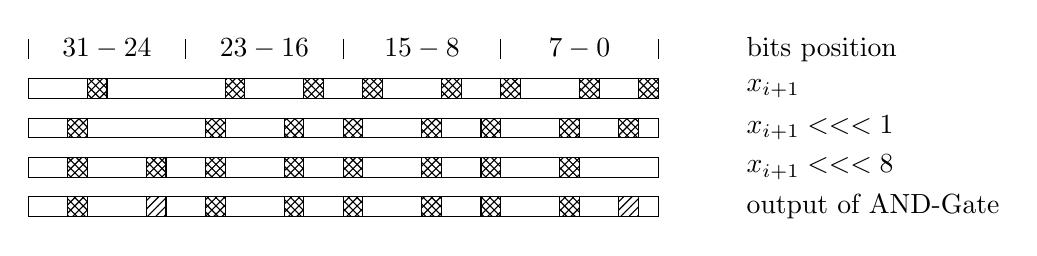
\begin{tikzpicture}	
	%\node[align=left, anchor=south west] at (0, 1.75) {$31$};
	%\node[align=left, anchor=south east] at (8, 1.75) {$0$};
	
	\node at (1, 2.125) {$31-24$};
	\node at (3, 2.125) {$23-16$};
	\node at (5, 2.125) {$15-8$};
	\node at (7, 2.125) {$7-0$};
	\node[align=left, anchor=west] at (9, 2.125) {bits position};
	
	\draw (0,2) -- (0, 2.25);
	\draw (2,2) -- (2, 2.25);
	\draw (4,2) -- (4, 2.25);
	\draw (6,2) -- (6, 2.25);
	\draw (8,2) -- (8, 2.25);
	
	\node[align=left, anchor=west] at (9, 1.625) {$x_{i+1}$};	\draw[pattern=crosshatch] (7.75, 1.5) rectangle (8,1.75);	
	\draw[pattern=crosshatch] (6, 1.5) rectangle (6.25,1.75);	
	\draw[pattern=crosshatch] (4.25, 1.5) rectangle (4.5,1.75);	
	\draw[pattern=crosshatch] (2.5, 1.5) rectangle (2.75,1.75);	
	\draw[pattern=crosshatch] (0.75, 1.5) rectangle (1,1.75);	
	\draw[pattern=crosshatch] (7, 1.5) rectangle (7.25,1.75);	
	\draw[pattern=crosshatch] (5.25, 1.5) rectangle (5.5,1.75);	
	\draw[pattern=crosshatch] (3.5, 1.5) rectangle (3.75,1.75);	
	\draw (0,1.5) rectangle (8,1.75);	
	
	\node[align=left, anchor=west] at (9, 1.125) {$x_{i+1} <<< 1$};
	\draw[pattern=crosshatch] (7.5, 1) rectangle (7.75,1.25);	
	\draw[pattern=crosshatch] (5.75, 1) rectangle (6,1.25);	
	\draw[pattern=crosshatch] (4, 1) rectangle (4.25,1.25);	
	\draw[pattern=crosshatch] (2.25, 1) rectangle (2.5,1.25);	
	\draw[pattern=crosshatch] (0.5, 1) rectangle (0.75,1.25);	
	\draw[pattern=crosshatch] (6.75, 1) rectangle (7,1.25);	
	\draw[pattern=crosshatch] (5, 1) rectangle (5.25,1.25);	
	\draw[pattern=crosshatch] (3.25, 1) rectangle (3.5,1.25);
	\draw (0,1) rectangle (8,1.25);	
	
	\node[align=left, anchor=west] at (9, 0.625) {$x_{i+1} <<< 8$};
	\draw[pattern=crosshatch] (5.75, 0.5) rectangle (6,0.75);	
	\draw[pattern=crosshatch] (4, 0.5) rectangle (4.25,0.75);	
	\draw[pattern=crosshatch] (2.25, 0.5) rectangle (2.5,0.75);	
	\draw[pattern=crosshatch] (0.5, 0.5) rectangle (0.75,0.75);	
	\draw[pattern=crosshatch] (6.75, 0.5) rectangle (7,0.75);	
	\draw[pattern=crosshatch] (5, 0.5) rectangle (5.25,0.75);	
	\draw[pattern=crosshatch] (3.25, 0.5) rectangle (3.5,0.75);
	\draw[pattern=crosshatch] (1.5, 0.5) rectangle (1.75,0.75);
	\draw (0,0.5) rectangle (8,0.75);	
	
	\node[align=left, anchor=west] at (9, 0.125) {output of AND-Gate};
	\draw[pattern=north east lines] (7.5, 0) rectangle (7.75,0.25);	
	\draw[pattern=crosshatch] (5.75, 0) rectangle (6,0.25);	
	\draw[pattern=crosshatch] (4, 0) rectangle (4.25,0.25);	
	\draw[pattern=crosshatch] (2.25, 0) rectangle (2.5,0.25);	
	\draw[pattern=crosshatch] (0.5, 0) rectangle (0.75,0.25);	
	\draw[pattern=crosshatch] (6.75, 0) rectangle (7,0.25);	
	\draw[pattern=crosshatch] (5, 0) rectangle (5.25,0.25);	
	\draw[pattern=crosshatch] (3.25, 0) rectangle (3.5,0.25);
	\draw[pattern=north east lines] (1.5, 0) rectangle (1.75,0.25);
	
	%\draw[pattern=north east lines] (4,0) rectangle (5.75,0.25);
	%\draw[pattern=crosshatch] (5.75,0) rectangle (6,0.25);
	%\draw[pattern=north east lines] (6,0) rectangle (7.75,0.25);
	\draw (0,0) rectangle (8,0.25);	
	
\end{tikzpicture} 


	\caption{Good choice for guessing 8 bits when attacking the AND-Gate. The guessed bits are distributed with a distance of 7 and therefore mostly line up at the AND-Gate.}
	\label{fig:goodExample}
\end{figure}

\paragraph{Attack steps} The CPA attack was executed according to the following procedure:
\begin{enumerate}
	\item Collect $n$ power traces with $m$ samples each. The whole measurement is a tuple $(T, P, C)$. $T$ is a Matrix of size $(n,m)$ which contains all traces. $P$ contain the plaintexts $p_i$ and $C$ contains the ciphertexts $c_i$.
	$$T
	=
	\begin{pmatrix}
		t_{1,1}& \cdots& t_{1,m} \\
		\vdots & & \vdots \\
		t_{n,1}& \cdots& t_{n,m} \\
	\end{pmatrix}	
	\quad P = 	\begin{pmatrix}
		p_1 \\
		\vdots\\
		p_n
	\end{pmatrix}
	\quad C = 	\begin{pmatrix}
		c_1 \\
		\vdots\\
		c_n
	\end{pmatrix}
	$$
	
	\item Create $2^b$ key candidates $K^*$. $b$ tells how many bits are guessed.
	
	$$K^*=
	\begin{pmatrix}
		k^*_1 \hdots k^*_{2^b}
	\end{pmatrix}
	$$
	% In later iterations, create key candidates based on key candidates that were marked as promising before. Adjust $B$ to mask all bits of the key which are guessed.
	
	\item For all combinations of plaintexts and key candidates, calculate the attacked intermediate state $x$. Calculate the hamming weight $hw$ of $x$ but only consider the bits which are influenced by the guessed key bits. The result is the matrix $HW$.
	$$
	HW =
	\begin{pmatrix}
		hw_{1,1}& \cdots& hw_{1,2^b} \\
		\vdots & & \vdots \\
		t_{n,1}& \cdots& t_{n,2^b} \\
	\end{pmatrix}
	$$
	
	\item Calculate the Pearson Correlation matrix between $HW^T$ and $T$. The results is a matrix $\rho$ with size $(2^b, m)$. Compute the matrix $\hat{\rho}$ by selecting the the element with the largest absolute value in each row. Compute the value $\tilde{\rho}$ by selecting the largest value of all $|\hat{\rho}_i|$.
	$$
	\rho = 
	\begin{pmatrix}
		\rho_{1,1}& \cdots& \rho_{1,m} \\
		\vdots & & \vdots \\
		\rho_{2^b,1}& \cdots& \rho_{2^b,m} \\
	\end{pmatrix}	
	\quad
	\hat{\rho} = 
	\begin{pmatrix}
		\hat{\rho}_{1}\\
		\vdots \\
		\hat{\rho}_{2^b}\\
	\end{pmatrix}	
	$$
	\item Based on a threshold $\tau$, find all values $\hat{\rho}_i$ where $|\hat{\rho}_i| + \tau \geq \tilde{\rho}$ The corresponding key candidates $k^*_i$ are marked as promising.
	\item For all promising key candidates, create sub candidates and repeat the process from step 3. With this approach, all possible key candidates form a tree where only promising paths are further processed.
	\item After attacking all 4 rounds, go through the remaining key candidates and check if encrypting the plaintext $p_1$ results in the corresponding ciphertext $c_1$.
\end{enumerate}

\paragraph{Attack Results}
The power traces clearly show the execution of the SIMON round functions (see Figure \ref{fig:power_graph_plain}). This is useful for the attack because the trace can be shortened to the first few rounds. In our experiments only the first 800 samples were included into the attack.

\begin{figure}[H]
	\centering
	\includegraphics[width=0.5\linewidth]{../simon/diagrams/power_graph_plain.pdf}
	\caption{Power consumption graph for the unprotected Simon implementation shows repeating patterns for the 44 rounds from sample 0 to approximately 2600.}
	\label{fig:power_graph_plain}
\end{figure}

Both attacks successfully recovered the full 128-bit key from the unprotected implementation. Figure \ref{fig:cpa_correlation_traces} shows the correlation traces for the correct key candidate and the 255 incorrect ones. For both attacks, the correct candidate has the highest correlation values. In the first attack, the inverse of each key candidate results in a mirrored correlation line. 

For the second attack, the graph is not symmetric. In the shown example, the correct key guess has a significantly higher correlation than the inverted one ($-0.471$ vs. $0.422$). However, this observation was not always true. In some rare cases, the inverted key had higher correlation values than the correct one. The root cause of this phenomenon is not investigated deeper in this work. 

\begin{figure}[H]
    \centering
    \begin{subfigure}{0.48\textwidth}
    	\centering
    	\includegraphics[width=\linewidth]{../simon/diagrams/correlation_over_time_plain.pdf}
    	\caption{Attack 1 (After adding key via XOR)}
    \end{subfigure}
    \begin{subfigure}{0.48\textwidth}
    	\centering
    	\includegraphics[width=\linewidth]{../simon/diagrams/correlation_over_time_andgate.pdf}
    	\caption{Attack 2 (After AND-Gate)}
    \end{subfigure}
    
    \caption{Correlation values over time for 256 key candidates with 50.000 traces.}
    \label{fig:cpa_correlation_traces}
\end{figure}

It was also analyzed how the correlation changes with an increasing number of captured traces. Figure \ref{fig:correlation_evolution_plain} shows the evolution for one measurement campaign and 8 bits being guessed. The experiments have shown that 1000 traces are enough to reliably extract the key.

For attack model 1, the correct key guess was always located within the Top 8 of all key guesses. Because of the symmetry, there are always at least 2 candidates that will be kept for the next attack round. The correlation threshold $\tau$ for marking a key candidate as promising was set to $0.02$.

For attack model 2, the correct key guess was often found as the top candidate, which is a slight advantage compared to model 1. However, in some cases, the correct key was only found within the Top 10. 
This might be caused by the fact, that instead of 8 bits, only 7 bits are included in the Hamming weight calculation (see chapter 2.2 and Figure \ref{fig:goodExample} for explanation).
The threshold $\tau$ was therefore increased to $0.03$ because otherwise the correct key might not be found.

The best performance was achieved with $4 \leq b \leq 8$, meaning 4 to 8 key bits are guessed in each attack step. With the chosen parameters, both attacks are equally reliable and have a similar performance. The correct key can be extracted on a standard computer within a few seconds.

\begin{figure}[H]
    \centering
    \begin{subfigure}{0.48\textwidth}
    	\centering
    	\includegraphics[width=\linewidth]{../simon/diagrams/correlation_over_num_measurements_plain.pdf}
    	\caption{Attack 1 (After adding key via XOR)}
    \end{subfigure}
    \begin{subfigure}{0.48\textwidth}
    	\centering
    	\includegraphics[width=\linewidth]{../simon/diagrams/correlation_over_num_measurements_andgate.pdf}
    	\caption{Attack 2 (After AND-Gate)}
    \end{subfigure}
    
    \caption{Maximum correlation values as the number of power traces increases.}
    \label{fig:correlation_evolution_plain}
\end{figure}

\section{Masking as a Countermeasure}
Boolean masking with two shares was implemented as a countermeasure. 184 random bytes are generated before the encryption using a PRNG based on HMAC (see \cite{barker2015recommendation}). 8 bytes of randomness are used to mask the plaintext via XOR. 4 additional bytes are required in each of the 44 rounds to perform the AND-operation. The binary rotations and XOR-operations within the round do not require additional masks. The operations can be performed independently on both shares.

Figure \ref{fig:simon_round_masked} shows the updated round function. The blue content is newly added compared to the original round function. The AND-Gate cannot be performed on both shares independently. The Trichina AND-Gate was implemented to avoid any leakage. The inputs of this AND-Gate are the shares of $a$ and $b$. Additionally, a new mask $m_c$ is brought in. 
$$
	a_m = a \oplus m_a \quad\quad b_m = b \oplus m_b
$$
The AND-Gate must generate the share $c_m$ such that:

$$
	c = a \cdot b \quad\rightarrow\quad c_m \oplus m_c = (a_m \oplus m_a) \cdot (b_m \oplus m_b)
$$
This equation is rearranged to the following form. It can be shown that all intermediate values in this formula are independent from the sensitive values $a$, $b$ and $c$. \cite{EPRINT:Trichina03}, \cite{trichina2004small}

$$
	c_m = (((a_m  b_m \oplus m_c) \oplus a_m m_b) \oplus b_m m_a) \oplus m_a m_b
$$

\begin{figure}[ht]
	\centering
	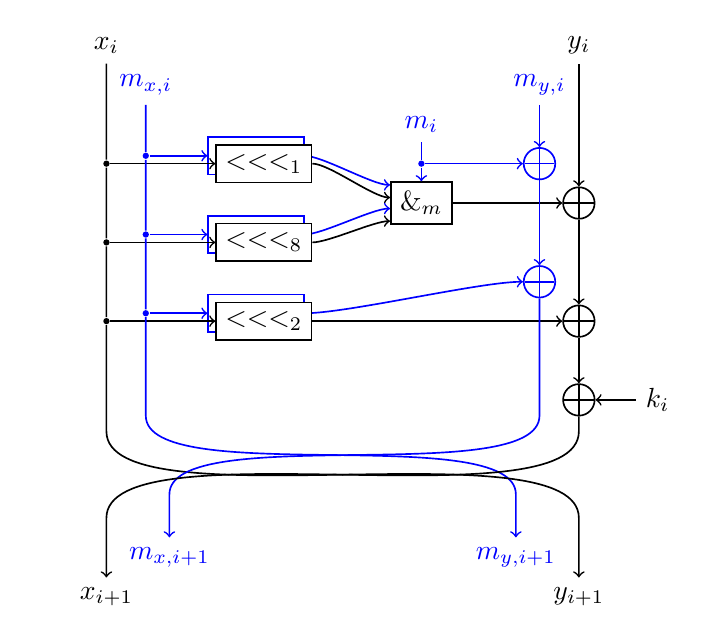
\begin{tikzpicture}
	[line width=0.6,trim left,
	box/.style = {
		draw,
		fill=white
	},
	loosewire/.style = {
		looseness=0.5,
	},
	xor/.style = {
		draw, circle, inner sep=0cm, minimum size=0.4cm,
		append after command = {
			[shorten >=\pgflinewidth, shorten <=\pgflinewidth,]
			(\tikzlastnode.north) edge (\tikzlastnode.south)
			(\tikzlastnode.east) edge (\tikzlastnode.west)
		}
	},
	xorblue/.style = {
		draw=blue, circle, inner sep=0cm, minimum size=0.4cm,
		append after command = {
			[shorten >=\pgflinewidth, shorten <=\pgflinewidth,]
			(\tikzlastnode.north) edge[draw=blue] (\tikzlastnode.south)
			(\tikzlastnode.east) edge[draw=blue] (\tikzlastnode.west)
		}
	},
	circ/.style = {
		draw, circle, inner sep=0cm, minimum size=0.4cm
	},
	dot/.style = {
		fill, circle, inner sep=0cm, minimum size=0.08cm
	}]
	
	%Draw nodes
	\node at (1,7.5) (xin) {$x_i$};
	\node[text=blue] at (1.5,7) (mx) {$m_{x,i}$};
	\node at (7,7.5) (yin) {$y_i$};
	\node[text=blue] at (6.5,7) (my) {$m_{y,i}$};
	\node[text=blue] at (5,6.5) (mi) {$m_i$};
	
	\node[dot,fill=blue] at (1.5,6.1) (d1m) {};
	\node[dot] at (1,6) (d1) {};
	\node[dot,fill=blue] at (1.5,5.1) (d2m) {};
	\node[dot] at (1,5) (d2) {};
	\node[dot,fill=blue] at (1.5,4.1) (d3m) {};
	\node[dot] at (1,4) (d3) {};
	
	\node[dot,fill=blue] at (5,6) (d4m) {};
	
	\node[box, draw=blue] at (2.9,6.1) (S1m) {$<<<_1$};
	\node[box] at (3,6) (S1) {$<<<_1$};
	\node[box, draw=blue] at (2.9,5.1) (S2m) {$<<<_8$};
	\node[box] at (3,5) (S2) {$<<<_8$};
	\node[box, draw=blue] at (2.9,4.1) (S3m) {$<<<_2$};
	\node[box] at (3,4) (S3) {$<<<_2$};
	
	\node[xorblue] at (6.5,6) (x1m) {};
	\node[xor] at (7,5.5) (x1) {};
	\node[xorblue] at (6.5,4.5) (x2m) {};
	\node[xor] at (7,4) (x2) {};
	\node[xor] at (7,3) (x3) {};
	
	\node[box] at (5,5.5) (AND) {$\&_m$};
	\node at (8,3) (k) {$k_i$};
	
	\node at (1, 0.5) (xout) {$x_{i+1}$};
	\node[text=blue] at (1.8, 1) (mxout) {$m_{x,i+1}$};
	
	\node at (7, 0.5) (yout) {$y_{i+1}$};
	\node[text=blue] at (6.2, 1) (myout) {$m_{y,i+1}$};
	
	\coordinate (cright) at (7, 2.6);
	\coordinate (cleft) at (1, 2.6);
	\coordinate (cright2) at (7, 1.5);
	\coordinate (cleft2) at (1, 1.5);
	\coordinate (crightm) at (6.5, 2.8);
	\coordinate (cleftm) at (1.5, 2.8);
	\coordinate (crightm2) at (6.2, 1.8);
	\coordinate (cleftm2) at (1.8, 1.8);
	
	%Draw wires
	\draw[->,draw=blue] (d1m) -- (S1m);
	\draw[->] (d1) -- (S1);
	
	\draw[loosewire,->,draw=blue] (S1m.east) to[out=0, in=180] (AND.150);
	\draw[loosewire,->] (S1.east) to[out=0, in=180] (AND.170);
	\draw[->,draw=blue] (d2m) -- (S2m);
	\draw[->] (d2) -- (S2);
	
	\draw[loosewire,->,draw=blue] (S2m.east) to[out=0, in=180] (AND.190);
	\draw[loosewire,->] (S2.east) to[out=0, in=180] (AND.210);
	
	\draw[->] (AND) -- (x1);
	
	\draw[->,draw=blue] (d3m) -- (S3m);
	\draw[->] (d3) -- (S3);
	
	\draw[loosewire,->,draw=blue] (S3m.east) to[out=0,in=180] (x2m);
	\draw[->] (S3.east) -- (x2);
	
	\draw[loosewire,->,draw=blue] (mx) -- (d1m) -- (d2m) -- (d3m)
	-- (cleftm) to[out=270, in=90] (crightm2) -- (myout.north);
	\draw[loosewire,->] (xin) -- (d1) -- (d2) -- (d3)
	-- (cleft) to[out=270, in=90] (cright2) -- (yout.north);
	
	
	\draw[->,draw=blue] (my) -- (x1m);
	\draw[->] (yin) -- (x1);
	\draw[->,draw=blue] (x1m) -- (x2m);
	\draw[->] (x1) -- (x2);
	\draw[->] (x2) -- (x3);
	
	\draw[loosewire,->,draw=blue] (x2m) -- (crightm) to[out=270, in=90] (cleftm2) -- (mxout.north);
	\draw[loosewire,->] (x3) -- (cright) to[out=270, in=90] (cleft2) -- (xout.north);
	\draw[->] (k.west) -- (x3);
	
	%additional wires for mask
	\draw[->,draw=blue] (mi) -- (d4m) -- (AND);
	\draw[->,draw=blue] (d4m) -- (x1m.west);
	
	%draw black boxes again to show them in front of blue arrows
	\node[box] at (3,6) (S1) {$<<<_1$};
	\node[box] at (3,5) (S2) {$<<<_8$};
	\node[box] at (3,4) (S3) {$<<<_2$};
	
\end{tikzpicture} 


	\caption{One round of the masked Simon implementation}
	\label{fig:simon_round_masked}
\end{figure}

\paragraph{Avoiding Pitfalls} The masked implementation was written in Assembly language (ASM). Potential hamming distance leakage was taken into account during implementation. Literature shows that updating a CPU register will leak the hamming distance between old and new value. Also, performing two arithmetic instructions in a row leaks the hamming distance between input/output operands, even if different CPU registers are used in the two instructions. \cite{seuschek2015side}, \cite{CHES:BriClaOli04}

To avoid leaking confidential information, following precautions were taken:
\begin{itemize}
	\item Masked values and the masks itself shall be stored in separated registers. In our implementation, even register numbers were used for masked values and odd registers for masks.
	\item Masked values and their corresponding masks shall not be processed in two consecutive instructions. Therefore, dummy instructions were added to clear values within the arithmetic logical unit (ALU).
	\item Intermediate values which occur, e.g., during the Trichina-AND-Gate, shall be cleared before being reused again.
\end{itemize}

\begin{figure}[H]
	\centering
	\includegraphics[width=0.5\linewidth]{../simon/diagrams/power_graph_masked.pdf}
	\caption{In this graph, 25 of the 44 rounds are visible. Each round takes approximately 4 times as long compared to the unmasked implementation.}
	\label{fig:power_graph_masked}
\end{figure}

\paragraph{Attack on the masked implementation}
The attacks were repeated on the masked implementation using 50,000 traces. At no point in time, the correct key candidate stands out from the other key candidates. With an increasing number of traces, the maximum correlation goes close to zero. (see Figure \ref{fig:masked_attack})
\begin{figure}[H]
    \centering
    \begin{subfigure}{0.48\textwidth}
        \centering
        \includegraphics[width=\linewidth]{../simon/diagrams/correlation_over_time_masked.pdf}
        \caption{Correlation over time during the first 4 rounds with 50.000 traces.}
    \end{subfigure}
    \hfill
    \begin{subfigure}{0.48\textwidth}
        \centering
        \includegraphics[width=\linewidth]{../simon/diagrams/correlation_over_num_measurements_masked.pdf}
        \caption{Maximum correlation values as the number of traces increases.}
    \end{subfigure}
    \caption{Attack results on masked Simon implementation.}
    \label{fig:masked_attack}
\end{figure}

\section{Statistical Leakage Assessment}
\paragraph{Methodology}
Welch's t-test (Test Vector Leakage Assessment, TVLA) was employed to detect leakage in both unprotected and masked implementations. Two sets of traces were collected in an alternating way:
\begin{itemize}
    \item \textbf{Set 1:} Fixed key, fixed plaintext
    \item \textbf{Set 2:} Fixed key, random plaintexts
\end{itemize}

The t-value was computed for each time sample between set 1 and set 2. A threshold of \(|t|>4.5\) indicates that the mean power consumption in set 1 is significantly different from set 2 with 99.999\% confidence \cite{gilbert2011testing}. In a perfect implementation, the mean values of set 1 and 2 should be equal at every point in time. Therefore a high t-value is a indicator that confidential information might be leaked.

\paragraph{Results}
The t-value over time can be seen in Figure \ref{fig:leakage}.
\begin{itemize}
    \item \textbf{Unprotected Simon:} Strong leakage was detected with t-values exceeding 600 at multiple time points, confirming high vulnerability to CPA attacks.
    \item \textbf{Masked Simon:} The t-values remained below the threshold for most of the samples. However, at the beginning of round 1, the t-values are outside the expected range. Additionally, there are some samples at later rounds where $|t|$ is larger than $4.5$.
    The t-values at the beginning are likely caused by hamming distance leakage at the beginning of round 1. The unmasked plaintext is still present in a CPU register before it is cleared in explicitly in an assembly instruction. This is uncritical for a CPA because no confidential values are being processed at that time. This hypothesis is supported by the fact that later SIMON rounds use the identical code but do not show such a high t-value.
    
\end{itemize}

\begin{figure}[H]
	\centering
    \begin{subfigure}{0.48\textwidth}
    	\centering
    	\includegraphics[width=\linewidth]{../simon/diagrams/leakage_over_time_plain.pdf}
    	\caption{Unprotected Implementation}
    \end{subfigure}
    \begin{subfigure}{0.48\textwidth}
    	\centering
    	\includegraphics[width=\linewidth]{../simon/diagrams/leakage_over_time_masked.pdf}
    	\caption{Masked Implementation}
    \end{subfigure}
    \caption{T-Value over time in the unprotected and masked Simon implementations}
    \label{fig:leakage}
\end{figure}


\section{Conclusion}
This study demonstrates that an unprotected software implementation of SIMON-64/128 is highly vulnerable to Correlation Power Analysis, enabling full key recovery with 1000 power traces. The application of Boolean masking made the original attack fail and drastically reduced leakage. However, the t-values are not completely within the desired threshold of $4.5$.

Our results demonstrate a clear trade-off between security and performance in lightweight cryptography implementations. This highlights several important considerations:

\begin{itemize}
	\item \textbf{Implementation quality:} The effectiveness of masking depends heavily on proper implementation, including secure random number generation avoiding hamming distance leakage.
	\item \textbf{Other Attack methods:} While the original attack was not successful on the masked implementations, other approaches like Higher-Order CPA might still be possible.
	\item \textbf{Performance overhead:} The masking implementation increased the encryption time by factor 4. Additional time is required for generating the random numbers. This may be acceptable for many IoT applications but could be prohibitive for extremely resource-constrained devices.
\end{itemize}

Future work should investigate higher-order masking schemes and their practical applicability to resource-constrained devices, as well as combining masking with alternative countermeasures.

The performance of generating the random numbers was not in the scope of this paper. For real-world use cases, one should investigate if faster random number generators have an impact on the security and if masks can be reused in multiple rounds.

When implementing lightweight cryptography devices, we recommend:
\begin{itemize}
    \item Evaluate the overall security of the hardware. Securing a device against side-channel attacks might not make sense if the device offers simpler attack vectors (e.g. unlocked JTAG interface)
    \item Use widespread techniques like T-Test to evaluate leakage. Do not classify a implementation as secure just because the original attack is not working anymore.
    \item Consider the trade-offs between security, performance, and resource constraints when selecting countermeasures.
    \item Stay updated on new attack techniques and countermeasures.
\end{itemize}

\appendix
\section{Measurement Parameters}
\begin{table}[H]
\centering
\begin{tabular}{ll}
\toprule
\textbf{Parameter} & \textbf{Value} \\
\midrule
Microcontroller & STM32F303 (ARM Cortex-M4) \\
Clock frequency & 7.38 MHz \\
Sampling rate & 29.5 MS/s \\
Samples per trace & 5,000 \\
Traces per Measurement & 50,000 \\
TVLA threshold & ±4.5 \\
\bottomrule
\end{tabular}
\caption{Experimental measurement parameters}
\label{tab:params}
\end{table}

\bibliographystyle{alpha}
\bibliography{abbrev3,crypto,biblio}


%\begin{thebibliography}{99}
%\bibitem{simon2013}
%Beaulieu, R., Shors, D., Smith, J., Treatman-Clark, S., Weeks, B., \& Wingers, L. (2013). The SIMON and SPECK Families of Lightweight Block Ciphers. \textit{CRYPTOLOGY EPRINT ARCHIVE}.

%\bibitem{cpa2004}
%Brier, E., Clavier, C., \& Olivier, F. (2004). Correlation Power Analysis with a Leakage Model. \textit{International Workshop on Cryptographic Hardware and Embedded Systems}.

%\bibitem{tvla2011}
%Goodwill, G., Jun, B., Jaffe, J., \& Rohatgi, P. (2011). A testing methodology for side-channel resistance validation. \textit{NIST non-invasive attack testing workshop}.

%\bibitem{trichina2003}

%\end{thebibliography}


\end{document}
